\chapter{Asymptotic Safety of Gravity-Matter Systems}
For computing the contributions of the different matter fields on the running of the cosmological constant and the Newton coupling we follow \cite{DonaEichhornPercacci2013}. 


Some important formulas:
\begin{align}
	\eta_{\Psi} = -\partial_t \ln Z_{\Psi}
\end{align}

\begin{align}
	R_{k, \Psi}(z) = Z_{\Psi} \ \mathbbm{1} \ z \ r\left(\frac{z}{k^2}\right)
\end{align}
where $r$ is the same Litim-type shape function as defined in (\ref{eqn:Litim}).
\section{Matter Contributions from Background Field Computation}
\begin{align}
	\Gammak = \Gamma_{\text{EH}} + \mathcal{S}_{\text{gf}}+ \mathcal{S}_{\text{gh}}+ \Gamma_{\text{matter}}
\end{align}
where the different matter contributions come from
\begin{align}
	\Gamma_{\text{matter}} = \mathcal{S}_{\text{S}} + \mathcal{S}_{\text{D}} + \mathcal{S}_{\text{V}} 
\end{align}
with 
\begin{align}
	\mathcal{S}_{\text{S}} &= \frac{Z_{\text{S}}}{2}\int_x \sqrt{\operatorname{det}g} \ g^{\mu\nu} \ \sum\limits_{i=1}^{N_{\text{S}}} \partial_{\mu}\phi^{i}\partial_{\nu}\phi^{i} \\
	\phantom{.}\nonumber\\
	\mathcal{S}_{\text{D}} &= iZ_{\text{D}}\int_x \sqrt{\operatorname{det}g} \ \sum\limits_{i=1}^{N_{\text{D}}} \bar{\psi}^{i}\slashed{\nabla}\psi^{i}\\
	\phantom{.}\nonumber\\
		\mathcal{S}_{\text{V}} &= \frac{Z_{\text{V}}}{4}\int_x \sqrt{\operatorname{det}g} \ \sum\limits_{i=1}^{N_{\text{V}}} g^{\mu\nu}g^{\kappa\lambda}F^{i}_{\mu\kappa}F^{i}_{\nu\lambda} \nonumber \\
		&+ \frac{Z_{\text{V}}}{2\xi}\int_x \sqrt{\operatorname{det}\bar{g}} \ \sum\limits_{i=1}^{N_{\text{V}}} \left(\bar{g}^{\mu\nu}\bar{D}_{\mu}A_{\nu}^{i}\right)^2  \\
		&+ \frac{1}{2}\int_x \sqrt{\operatorname{det}\bar{g}} \ \sum\limits_{i=1}^{N_{\text{V}}} \bar{c}_i(-\bar{D}^2)c_i \nonumber
\end{align}
\begin{figure}[H]
	\centering
	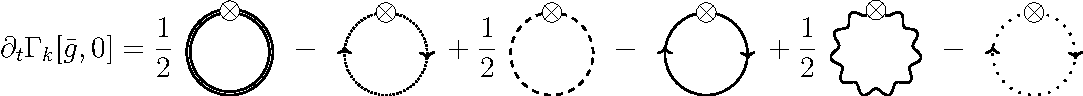
\includegraphics[width=0.95\textwidth]{figs/TikZ/matter_corrections}
	\caption[Flow equation for the average effective action $\Gamma_k$ including different matter contributions in diagrammatic representation.]{Flow equation for the average effective action $\Gamma_k$ including different matter contributions in diagrammatic representation. The double, dashed, solid and  wiggly lines correspond to the graviton, scalar, fermion and gauge field  propagators, respectively. The crossed circles denote the insertion of the respective regulator.}
\end{figure}

\begin{itemize}
	\item wo essential couplings, $G$ and $\Lambda$ and five inessential\footnote{Inessential in this sense means, that they can be eliminated by field rescalings.} wave function renormalizations $Z_{\Psi}$ with $\Psi = (h,c,S,D,V)$.
\end{itemize}
\subsection{Scalar fields}
\begin{align}
	\mathcal{S}_S &= \frac{Z_{S}}{2}\int_x \sqrt{\operatorname{det}g} \ g^{\mu\nu} \ \sum\limits_{i=1}^{N_{\text{S}}} \partial_{\mu}\phi^{i}\partial_{\nu}\phi^{i} \nonumber \\
&=  \frac{Z_{S}}{2}\int_x \sqrt{\operatorname{det}\bar{g}} \ \bar{g}^{\mu\nu} \ \sum\limits_{i=1}^{N_{\text{S}}} \partial_{\mu}\phi^{i}\partial_{\nu}\phi^{i} + \mathcal{O}(h) \\
&\overset{(\star)}{=} \frac{Z_{S}}{2}\int_x \sqrt{\operatorname{det}\bar{g}} \ \ \sum\limits_{i=1}^{N_{\text{S}}} \phi^{i}\left(-\bar{\nabla}^2\right)\phi^{i} + \mathcal{O}(h) \nonumber
\end{align}

Two-point function:
\begin{align}
	\Gamma^{(2)}_{\phi\phi} = \frac{\delta^2 \mathcal{S}_S}{\delta\phi^{i}\ \delta\phi^{j}} = Z_S \cdot\bar{\Delta}\cdot\mathbbm{1}_S + \mathcal{O}(h)  
\end{align}

Regularized Two-Point-Function:
\begin{align}
	\Gamma^{(2)}_{k, \phi\phi} = \left[\Gamma^{(2)}_{\phi\phi}+ R_{k, S}\right]  = Z_S \cdot\bar{\Delta}\cdot\mathbbm{1}_S\left(1 + r_k\left(\frac{\bar{\Delta}}{k^2}\right)\right) 
\end{align}



RHS of the flow equation:
\begin{align}
	\frac{1}{2}\tr{\left(\Gamma^{(2)}_{k, \phi\phi}\right)^{-1}\partial_t R_{k,S}} &= \frac{1}{2}\tr{\frac{Z_S\bar{\Delta}\left(\partial_t r_k - \eta_s r_k\right)}{Z_S \bar{\Delta}\left(1 + r_k\right)}\mathbbm{1}_S} \nonumber\\
	\phantom{.} \\
	&=   \frac{N_S}{2}\tr{\frac{Z_S\bar{\Delta}\left(\partial_t r_k - \eta_s r_k\right)}{Z_S \bar{\Delta}\left(1 + r_k\right)}} \nonumber
\end{align}

\subsection{Fermionic  fields}

\subsection{Gauge fields}
\begin{align}
	\mathcal{S}_{V, \mathrm{tot}} &= \frac{Z_{\text{V}}}{4}\int_x \sqrt{\operatorname{det}g} \ \sum\limits_{i=1}^{N_{\text{V}}} g^{\mu\nu}g^{\kappa\lambda}F^{i}_{\mu\kappa}F^{i}_{\nu\lambda}  
		+ \frac{Z_{\text{V}}}{2\xi}\int_x \sqrt{\operatorname{det}\bar{g}} \ \sum\limits_{i=1}^{N_{\text{V}}} \left(\bar{g}^{\mu\nu}\bar{D}_{\mu}A_{\nu}^{i}\right)^2  \nonumber\\
		&+ \frac{1}{2}\int_x \sqrt{\operatorname{det}\bar{g}} \ \sum\limits_{i=1}^{N_{\text{V}}} \bar{c}_i(-\bar{D}^2)c_i 
\end{align}



standard gauge field term:
\begin{align}
\mathcal{S}_{V} &=  \frac{Z_V}{4}\int_x \sqrt{\operatorname{det}g} \ \sum\limits_{i=1}^{N_{\text{V}}} g^{\mu\nu}g^{\kappa\lambda}F^{i}_{\mu\kappa}F^{i}_{\nu\lambda} \nonumber \\
&=  \frac{Z_{V}}{4}\int_x \sqrt{\operatorname{det}\bar{g}} \ \sum\limits_{i=1}^{N_{\text{V}}} \bar{g}^{\mu\nu}\bar{g}^{\kappa\lambda}\bar{F}^{i}_{\mu\kappa}\bar{F}^{i}_{\nu\lambda} + \mathcal{O}(h) \\
&\overset{(\ref{eqn:FF2})}{=} \frac{Z_{V}}{2}\int_x \sqrt{\operatorname{det}\bar{g}} \ \sum\limits_{i=1}^{N_{\text{V}}} A_{\lambda}^{i}\left[ \bar{g}^{\mu\lambda}\bar{\nabla}^{\mu}\bar{\nabla}^{\lambda} + \bar{\Delta}\right]A_{\mu}^{i} + \mathcal{O}(h) \nonumber
\end{align}
%TODO: Fix reference
gauge fixing term:
\begin{align}
	\mathcal{S}_{V, \mathrm{gf}} &= \frac{Z_{\text{V}}}{2\xi}\int_x \sqrt{\operatorname{det}\bar{g}} \ \sum\limits_{i=1}^{N_{\text{V}}} \left(\bar{g}^{\mu\nu}\bar{\nabla}_{\mu}A_{\nu}^{i}\right)^2  \nonumber\\
	&= \frac{Z_{\text{V}}}{2\xi}\int_x \sqrt{\operatorname{det}\bar{g}} \ \sum\limits_{i=1}^{N_{\text{V}}} \bar{g}^{\mu\nu}\bar{\nabla}_{\mu}A_{\nu}^{i}g^{\kappa\lambda}\bar{\nabla}_{\kappa}A_{\lambda}^{i} \\
	&\overset{(\star)}{=} \frac{Z_{\text{V}}}{2\xi}\int_x \sqrt{\operatorname{det}\bar{g}} \ \sum\limits_{i=1}^{N_{\text{V}}} A_{\lambda}^{i}\left[-\bar{\nabla}^{\lambda}\bar{\nabla}^{\mu}\right]A_{\mu}^{i} \nonumber
\end{align}
Both together 
Ghosts have to be considered separately \dots


\section{Perturbative Approximation}

\section{Some Words on Fermionic fields}
This section is mainly based on \cite{LippoldtPHD} and \cite{Lippoldt2015} where the spin-base invariant formalism for treating fermions in curved spacetimes has been developed. The goal of this part of the thesis is to get a rough idea on how to perform calculations involving Dirac fermions, especially in the context of Asymptotic Safety of gravity-matter systems.  

Covariant derivative:
\begin{align}
	\nabla_{\mu} = \partial_{\mu} + \frac{1}{8}\left[\gamma^{a}, \gamma^{b}\right]\omega_{\mu}^{ab}
\end{align}


 \begin{figure}[t]
 \centering
 \hfill
 \begin{subfigure}{0.3\textwidth} 
	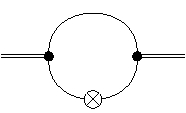
\includegraphics[width=\textwidth]{figs/TikZ/fermion_contribution}
 	\subcaption{Fermions.}
 \end{subfigure}
 \hfill
 \begin{subfigure}{0.3\textwidth} 
 	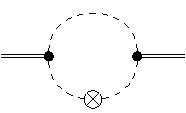
\includegraphics[width=\textwidth]{figs/TikZ/scalar_contribution}
 	\subcaption{Scalars.}
 \end{subfigure} 
 \hfill
 \begin{subfigure}{0.3\textwidth} 
 	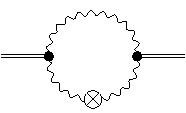
\includegraphics[width=\textwidth]{figs/TikZ/gauge_field_contribution}
 	\subcaption{Gauge Fields.}
 \end{subfigure} 
 \hfill
 \caption{Different matter contributions to the graviton anomalous dimension $\eta_h$.}	
 \end{figure}
 

 
  \begin{figure}[t]
 \centering
 \hfill
 \begin{subfigure}{0.3\textwidth} 
	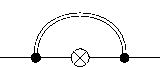
\includegraphics[width=\textwidth]{figs/TikZ/graviton_fluctuations1}
 \end{subfigure}
 \hfill
 \begin{subfigure}{0.3\textwidth}
 \vspace{-3.5pt}
 	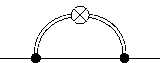
\includegraphics[width=\textwidth]{figs/TikZ/graviton_fluctuations2}
 \end{subfigure} 
 \hfill
 \begin{subfigure}{0.3\textwidth} 
 	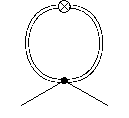
\includegraphics[scale = 1.5]{figs/TikZ/graviton_fluctuations3}
 \end{subfigure} 
 \hfill
 \caption[Contributing diagrams to the fermion anomalous dimension $\eta_D$.]{Contributing diagrams to the fermion anomalous dimension $\eta_D$. Analogous contributions arise for external scalars and gauge fields to $\eta_S$ and $\eta_V$.} 	
 \end{figure}
 
 \section{Background Field versus Fluctuation Field Calculation}

 